%%%%%%%%%%%%%%%%%%%%%%%%%%%%%%%%%%%%%%%%%%%%%%%%%%%%%%%%%%%%%%%
%
% ALERT --- *ACL (ACL Rolling Review) anonymous submission (main driver)
%
% Change "review" to "final" for the camera-ready, or to "preprint"
% for a non-anonymous version with page numbers.
%
%%%%%%%%%%%%%%%%%%%%%%%%%%%%%%%%%%%%%%%%%%%%%%%%%%%%%%%%%%%%%%%

\documentclass[11pt]{article}

% ACL style (loads natbib, caption, hyperref, and line numbers in review mode).
\usepackage[review]{acl}

% Standard fonts / encoding recommended by the ACL template.
\usepackage{times}
\usepackage{latexsym}
\usepackage[T1]{fontenc}
\usepackage[utf8]{inputenc}
\usepackage{microtype}
\usepackage{graphicx}

% ---------------------------------------------------------------
% Math, symbols, and tables
% ---------------------------------------------------------------
\usepackage{amsmath}
\usepackage{amssymb}
\usepackage{amsfonts}
\usepackage{amsthm}
\usepackage{booktabs}
\usepackage{multirow}
\usepackage{makecell}

% Algorithms
\usepackage{algorithm}
\usepackage{algorithmic}

% Lists, inline symbols, and code/quote boxes
\usepackage{enumitem}
\usepackage{textcomp}
\usepackage{xcolor}
\usepackage[most]{tcolorbox}

% Code/quote box for verbatim-like illustrative blocks
% (History, Progress Notes, prompt schematic)
\newtcolorbox{mycodebox}{
    enhanced,
    colback=gray!5,
    colframe=gray!40,
    arc=3mm,
    boxrule=0.8pt,
    left=2pt, right=2pt,
    top=4pt, bottom=4pt,
    width=\columnwidth,
    boxsep=0pt,
    halign=left
}

% TikZ for the (vectorized) architecture figure
\usepackage{tikz}
\usetikzlibrary{positioning,arrows.meta,fit,backgrounds,calc}

% Theorem-like environments
\newtheorem{proposition}{Proposition}

% ---------------------------------------------------------------
% Title and (anonymous) author block.
% In [review] mode the ACL style automatically prints
% "Anonymous ACL submission" and hides the author block below.
% ---------------------------------------------------------------
% Title alternatives kept for reference (uncomment to swap):
% \title{ALERT: An Agentic Framework for Proactive Legal Risk Intelligence in AI Product Development}
% \title{ALERT: Goal-Conditioned Agentic Risk Intelligence for AI Litigation}
% \title{ALERT: Proactive Legal Risk Intelligence via Goal-Conditioned Agentic Systems}

\title{ALERT: Goal-Conditioned Agentic Systems for Self-Verifying Risk Intelligence}

% In [review] mode the ACL style prints "Anonymous ACL submission" and
% suppresses this block. For the camera-ready (\usepackage{acl}), replace
% the placeholders below with the real author names and affiliations.
\author{
  Anonymous ACL submission \\
  \texttt{email@domain} \\
}


\begin{document}

\maketitle

% Force-include the case-study references that are discussed by name in
% the body but not formally \cite{}d inline.
\nocite{getty_stability_2023,
        nyt_openai_2023,
        kosari_meta_2024}

\begin{abstract}
We present ALERT (Agentic Legal Exposure and Risk Tracking), a deployable framework for turning fast-moving AI litigation into product-level risk intelligence. Its central AI mechanism is not an agent wrapper but a \emph{retrieval-time point-in-time authority gate}: a supersession-aware temporal precedent graph converts validity intervals and treatment edges into a scoring operator that changes the evidence distribution before generation. ALERT defines Product--Litigation Risk Entailment (PLRE), a directional task asking whether product attributes entail exposure to legal-risk theories under time-valid precedent, and implements a goal-conditioned loop whose stopping rule controls \emph{evidence coverage} rather than legal correctness. On ALERT-Dataset, the full system improves over rule-based, single-pass LLM, RAG-only, single-agent, compute-matched self-refinement, and non-ALERT PLRE baselines; the ordering persists on the human-adjudicated subset used as the primary circularity check. Ablations show that validity gating reduces stale citations and improves PLRE F1 relative to flat similarity. We release label provenance, annotation guidance, evaluation scripts, and an operational implementation. ALERT is decision support for qualified reviewers, not legal advice.
\end{abstract}


\section{Introduction}

Generative-AI products increasingly face litigation over training data, output reproduction, model behavior, and downstream misuse. For engineering organizations, the operational question is not merely whether a lawsuit exists, but whether a theory of liability maps to a product attribute, whether the supporting authority was valid at the relevant filing date, and which mitigation should be reviewed by counsel. Keyword alerts surface noisy filings, docket trackers rarely map cases to features, and conventional retrieval-augmented generation (RAG)~\citep{lewis2020retrieval} treats semantically similar legal documents as comparable even when later decisions have narrowed or superseded them.

We introduce ALERT (\textbf{Agentic Legal Exposure and Risk Tracking}), a continuous sensing system for AI-litigation risk intelligence. ALERT combines CourtListener/RECAP and legal-news ingestion, a 22-field legal-ops schema, and a goal-conditioned reporting loop, producing structured risk registers with citations, provenance, and mitigation candidates while preserving human accountability for legal conclusions.

The paper's main research object is \emph{Product--Litigation Risk Entailment} (PLRE): deciding whether product attributes entail exposure to a legal-risk theory under time-valid precedent. PLRE differs from standard legal textual entailment because the premise is a product attribute, the hypothesis is a risk theory, and the entailment relation is conditioned on a temporal precedent graph. ALERT's graph borrows the legal intuition behind citators such as Shepard's and KeyCite---authority changes over time---but implements a public-corpus, automatically extracted, time-indexed treatment layer and connects it to product-facing entailment rather than to retrospective case lookup.

ALERT is therefore not a legal-monitoring pipeline with an agentic wrapper. Its reusable AI contribution is a point-in-time retrieval operator that changes the candidate evidence distribution \emph{before} generation, rather than filtering citations after an LLM has already produced a report. This distinction matters because stale but lexically similar precedent can dominate ordinary RAG, while PLRE requires product-to-theory entailment under authority valid at the query date. The agentic layer is used to expose unmet evidence atoms and stop when calibrated coverage is satisfied; the novelty claim is the coupling of this verifiable stopping rule with a temporal authority gate whose form is not legal-specific---Eq.~\eqref{eq:tpg_score} applies to any time-stamped, supersession-bearing authority corpus.

Our contributions are: (1) a supersession-aware temporal retrieval mechanism with validity intervals and treatment-edge weighting exposed as a retrieval-time authority gate; (2) PLRE, an \emph{initial} product-conditioned legal-risk entailment benchmark with non-ALERT baselines and ablations separating temporal validity from flat similarity; (3) a goal-conditioned agentic system whose stopping rule controls evidence coverage, not legal correctness; (4) ALERT-Dataset with per-record label provenance, product-mapping annotation guidance, and a human-adjudicated primary circularity check; and (5) a 30-day deployment showing reproducible legal-ops integration.


\section{Background and Scope}

\textbf{Legal-risk monitoring for AI products.} Legal-ops teams track dockets, news, and internal product changes, but the bridge from litigation event to product-specific engineering action is often manual. Copyright litigation against generative-AI systems has grown sharply since 2022, challenging web-scale training data~\citep{henderson2023foundation,levendowski2018copyright} under theories spanning DMCA \S1202 information removal, direct infringement, and vicarious liability for outputs~\citep{grimmelmann2015copyright}. ALERT targets this product-facing layer: it is not a legal decision system, but a structured sensing and evidence-organization system for qualified human review.

\textbf{Agentic RAG with verifiable stopping.} LLM agent frameworks~\citep{yao2022react,shinn2023reflexion,langgraph2024} show iterative tool use helps multi-step tasks. Standard RAG runs a fixed retrieval plan; self-refinement iterates but stops when the model judges its own answer satisfactory. ALERT instead uses an explicit goal predicate over required fields, evidence support, and provenance: under stated attainability and monotone-retrieval assumptions the loop terminates or escalates unmet conditions, and calibrated thresholds control evidence-omission risk in the calibration setting, not the truth of legal labels.

\textbf{Legal NLP and temporal legal authority.} Legal NLP has studied legal judgment prediction, legal entailment, statutory reasoning, case retrieval, and citation-network modeling, mostly treating the corpus as a static collection. In litigation sensing, however, time matters: a precedent's relevance depends on whether it had been narrowed, vacated, superseded, or overruled at the filing date. ALERT's temporal precedent graph makes this validity condition explicit and exposes it to retrieval, entailment, and mitigation generation.

\textbf{Decision-support boundary.} ALERT emits risk intelligence, evidence summaries, and mitigation candidates with provenance and residual uncertainty; it does not provide legal advice, replace counsel, predict outcomes, or recommend business decisions.


\section{Problem Formulation}
\label{sec:formulation}

Let $\mathcal{D}=\{d_1,\ldots,d_n\}$ be public litigation documents with metadata and text, and let $P$ be a product specification describing architecture, data provenance, modality, and deployment context. ALERT returns a structured report $R^*$ and mitigation candidates $G^*$:
\begin{equation}
  R^* = \arg\max_{R\in\mathcal{R}} \text{Quality}(R,\mathcal{D},P)
  \quad\text{s.t.}\quad \mathcal{G}(R)=\textsc{True}.
\end{equation}
Quality is operationalized in evaluation, not optimized as one loss: correctness/completeness by severity-label F1 (RQ1), actionability/clarity by blinded report ratings (RQ2), and evidence sufficiency by the coverage loss $L_\tau$ (RQ6); $\mathcal{G}$ is the auditable goal predicate below. The hard case is a domain gap: product specs use engineering terms such as data pipelines and API distribution, while litigation documents use causes of action, procedural posture, and precedent. PLRE therefore tests a context-aware entailment problem: map engineering-language attributes to legal-risk theories while conditioning the support set on authority valid at the query date. Operational integrations establish deployability; the AI contribution is the retrieval-and-entailment mechanism, not the surrounding monitoring workflow.

\subsection{Goal-Conditioned Agentic Loop}
\label{sec:goal_checker}

ALERT treats report generation as goal-conditioned planning. The predicate is:
\begin{equation}
\label{eq:goal_predicate}
  \mathcal{G}(R)=\mathcal{G}_{\text{risk}}(R)\wedge\mathcal{G}_{\text{evidence}}(R)\wedge\mathcal{G}_{\text{guide}}(R),
\end{equation}
where $\mathcal{G}_{\text{risk}}$ requires every risk item to have a severity label, $\mathcal{G}_{\text{evidence}}$ requires at least $k$ supporting documents above relevance threshold $\tau$, and $\mathcal{G}_{\text{guide}}$ requires mitigation text for each High or Medium item. The controller chooses among \textsc{Search}, \textsc{Analyze}, \textsc{Summarize}, \textsc{Map}, \textsc{Verify}, and \textsc{Report}; the deterministic Goal Checker either terminates, emits a structured critique to close residual gaps, or escalates unmet conditions. For example, if a High-risk item has only one valid authority after gating, the critique records the missing theory, product attribute, jurisdiction, query date, and required evidence count; the Planner rewrites this into narrower precedent and entity queries rather than simply retrying the same prompt.

Let $\Phi(R_t)$ count the unmet atomic sub-conditions of $\mathcal{G}$ and let $L_\tau(c)=\mathbf{1}[\text{a retrievable High-risk theory in case }c\text{ is omitted from }R^*]$ be the coverage loss at evidence threshold $\tau$.
\begin{proposition}[Coverage-controlled stopping with escalation]
\label{prop:termination}
Under monotone evidence caching and attainable progress, $\Phi(R_t)$ is non-increasing, reaches zero in at most $\Phi(R_0)$ successful progress steps when all atoms are attainable, and otherwise returns the residual atoms at $T_{\max}$. If $\hat\tau$ is selected on exchangeable calibration cases by conformal risk control, then the next-case omission risk satisfies $\mathbb{E}[L_{\hat\tau}]\le\alpha$.
\end{proposition}
The first clause is only a bounded stopping-and-escalation guarantee; the second clause is the statistical risk-control mechanism that makes the loop useful for AI evaluation. It controls evidence coverage under the calibration distribution, not severity-label correctness, legal advice, or future temporal shift.

\subsection{Risk Scoring}

The agentic layer scores risk as $\text{RiskScore}(d_i,P,C)=f_\theta(\phi(d_i),\psi(P),\chi(C))$, where $C$ is precedent context retrieved by LegalRisk-RAG. The ingestion layer uses an additive scoring matrix (Table~\ref{tab:risk_matrix}, appendix) for real-time triage, with a critical-composite bonus when copyright and model-training evidence co-occur; this heuristic is treated as a baseline and never as ground truth.


\section{The ALERT Framework}
\label{sec:framework}
We present ALERT, a goal-conditioned agentic framework for proactive legal risk intelligence.
\subsection{System Overview}

Figure~\ref{fig:alert_arch} presents the architecture: a lightweight sensing pipeline populates evidence records, while the agentic layer plans, retrieves, verifies, and reports under a deterministic Goal Checker. The figure is included to show where the proposed retrieval-time authority gate enters the evidence path, not to claim novelty for the surrounding integrations.



\begin{figure}[t]
\centering
\resizebox{\linewidth}{!}{%
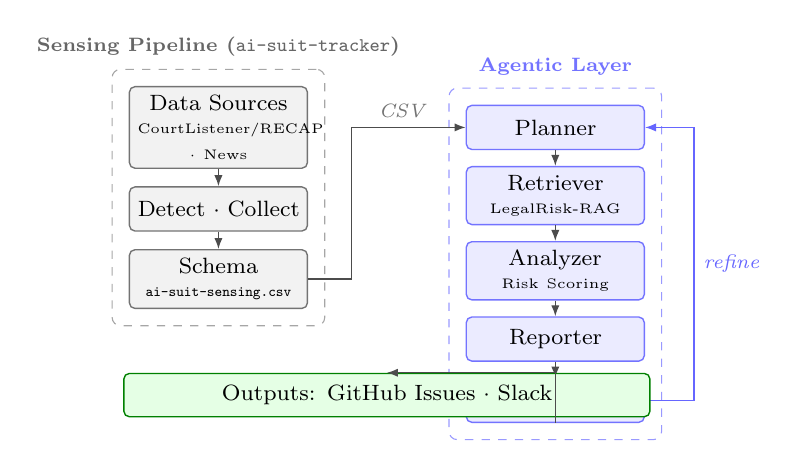
\begin{tikzpicture}[
  font=\footnotesize,
  box/.style={rectangle, rounded corners=2pt, draw, minimum height=0.56cm,
              align=center, inner sep=3pt, text width=2.05cm, line width=0.5pt},
  pipe/.style={box, fill=black!5, draw=black!55},
  agent/.style={box, fill=blue!8, draw=blue!55},
  outbox/.style={rectangle, rounded corners=2pt, draw=green!50!black, fill=green!10,
              align=center, inner sep=4pt, minimum height=0.55cm, text width=6.4cm, line width=0.5pt},
  arr/.style={-{Latex[length=1.4mm]}, draw=black!70, line width=0.5pt},
  lbl/.style={font=\scriptsize\itshape, text=black!55},
  grplab/.style={font=\scriptsize\bfseries, text=black!60}
]
% ---- left: sensing pipeline ----
\node[pipe] (ds) {Data Sources\\[-1pt]{\tiny CourtListener/RECAP $\cdot$ News}};
\node[pipe, below=0.22cm of ds] (sp) {Detect $\cdot$ Collect};
\node[pipe, below=0.22cm of sp] (sc) {Schema\\[-1pt]{\ttfamily\resizebox{1.85cm}{!}{ai-suit-sensing.csv}}};
\draw[arr] (ds) -- (sp);
\draw[arr] (sp) -- (sc);
% ---- right: agentic layer ----
\node[agent, right=2.0cm of ds] (pl) {Planner};
\node[agent, below=0.20cm of pl] (rt) {Retriever\\[-1pt]{\tiny LegalRisk-RAG}};
\node[agent, below=0.20cm of rt] (an) {Analyzer\\[-1pt]{\tiny Risk Scoring}};
\node[agent, below=0.20cm of an] (rp) {Reporter};
\node[agent, below=0.20cm of rp] (gc) {Goal Checker};
\draw[arr] (pl) -- (rt);
\draw[arr] (rt) -- (an);
\draw[arr] (an) -- (rp);
\draw[arr] (rp) -- (gc);
% schema feeds the agentic layer
\draw[arr] (sc.east) -- ($(sc.east)+(0.55,0)$) |- (pl.west) node[lbl, pos=0.72, above]{CSV};
% refine loop (Goal Checker -> Planner)
\draw[arr, draw=blue!60] (gc.east) -- ($(gc.east)+(0.62,0)$) |- (pl.east)
      node[lbl, text=blue!60, pos=0.25, right]{refine};
% ---- outputs ----
\node[outbox, below=0.42cm of $(sc)!0.5!(gc)$] (op) {Outputs: GitHub Issues $\cdot$ Slack};
\draw[arr] (gc.south) |- (op.north);
% ---- group containers ----
\begin{scope}[on background layer]
  \node[draw=black!35, dashed, rounded corners=3pt, inner sep=6pt, fit=(ds)(sp)(sc)] (gpipe) {};
  \node[draw=blue!40, dashed, rounded corners=3pt, inner sep=6pt, fit=(pl)(rt)(an)(rp)(gc)] (gag) {};
\end{scope}
\node[grplab, above=1pt of gpipe.north] {Sensing Pipeline (\texttt{ai-suit-tracker})};
\node[grplab, text=blue!55, above=1pt of gag.north] {Agentic Layer};
\end{tikzpicture}%
}
\caption{ALERT architecture. The sensing pipeline (left) detects filings, collects documents, and populates the schema; the agentic layer (right) plans, retrieves time-valid precedent, scores risk, and reports, with the Goal Checker driving a refine loop until evidence coverage is met.}
\label{fig:alert_arch}
\end{figure}

\subsection{Multi-Source Litigation Discovery and Schema Population}
\label{sec:discovery}

ALERT's discovery layer ingests CourtListener/RECAP~\citep{courtlistener2023}, docket-backed legal-media signals, and keyword-filtered news. A two-stage deduplication module first matches docket IDs and titles, then optionally removes Gemini-embedding neighbors above cosine $0.85$ (Algorithm~\ref{alg:hybrid_dedup}, appendix). Detected filings populate the 22-field \texttt{ai-suit-sensing.csv} schema by combining docket metadata, NER over complaint text, regex extraction for damages, and LLM summarization for the narrative fields.

\subsection{LegalRisk-RAG}

The LegalRisk-RAG pipeline adapts standard RAG to legal text in three ways. \textbf{Chunking} segments documents at \emph{logical structural boundaries}---numbered claims, ``WHEREFORE'' clauses, section headings---rather than fixed token windows, and each chunk retains a metadata header (case id, filing date, court level, section type). \textbf{Embedding}: we compared a dense retriever~\citep{karpukhin2020dense} (\texttt{text-embedding-3-large}), RECAP-tuned LegalBERT~\citep{chalkidis2020legalbert}, and a hybrid BM25 + neural re-ranker on a 200-pair development set; the hybrid (best) is the default (Table~\ref{tab:retriever_ablation}, appendix). \textbf{Dynamic context expansion (precedent chaining)}: when a retrieved chunk references a prior case (e.g., \emph{Authors Guild v.\ Google}), the pipeline appends that opinion as secondary context and queries the temporal precedent graph for subsequent treatment, so the Analyzer receives both semantic neighbors and validity metadata (cited positively, narrowed, superseded, or overruled at the filing date).

\subsection{Goal-Conditioned Agentic Loop}
\label{sec:agentic_loop}

The four specialized agents and the central Goal Checker operate as in Algorithm~\ref{alg:alert_loop}. The \textbf{Planner} decomposes unmet sub-goals into ordered retrieval/analysis sub-tasks; the \textbf{Retriever} runs LegalRisk-RAG queries and reformulates via legal entity term expansion when $\mathcal{G}_{\text{evidence}}$ is unmet; the \textbf{Analyzer} computes $\text{RiskScore}(d_i, P, C)$, clusters evidence, and maps clusters to a risk taxonomy (Training Data, Output Reproduction, API Misuse, Model Weights); the \textbf{Goal Checker} evaluates $\mathcal{G}(R_t)$ after each pass and returns machine-readable residuals such as \texttt{missing(valid-authority, DMCA, output-CMI, NDCA, 2025-02)}; the Planner converts these critiques into expanded entity/date/theory queries; and the \textbf{Reporter} assembles the risk register, per-risk evidence with citations, and mitigation guidance. The ingestion and risk-scoring components are released as \texttt{ai-suit-tracker} (anonymous review URL in the supplement), with configuration, prompt templates, and run parameters in the appendix.

\subsection{Supersession-Aware Temporal Precedent Graph}
\label{sec:tpg}

ALERT's central reusable mechanism is a retrieval-time authority gate implemented by a temporal precedent graph $\mathcal{P}_t=(V,E_t)$. Each node $v\in V$ denotes a case, order, or doctrinal rule and stores jurisdiction, court level, issue tags, filing/decision dates, and a validity interval $[s_v,e_v)$, where $e_v$ is open unless the node is later vacated, overruled, superseded, or materially narrowed. Directed edges encode treatment relations: \textsc{cites}, \textsc{distinguishes}, \textsc{narrows}, \textsc{supersedes}, and \textsc{overrules}. Retrieval for a query at date $t_q$ first obtains semantically relevant candidates and then applies validity gating:
\begin{equation}
\label{eq:tpg_score}
  \mathrm{score}(v,q,t_q)=\mathrm{sim}(v,q)\cdot \mathbf{1}[s_v\!\le\! t_q\!<\! e_v]\cdot w(\mathrm{treat}(v,t_q)).
\end{equation}
Here $w(\cdot)$ is a fixed, bounded monotone schedule in $(0,1]$: positively treated or still-open precedents take weight $1$, cautionary or materially narrowed authorities are down-weighted, and fully closed authorities are already removed by the indicator (the exact schedule is released with the implementation). This separates legal authority from topical similarity: a stale but lexically close case may be retrieved for context, but it cannot dominate the risk decision without passing the time-validity check. Algorithmically, Eq.~\eqref{eq:tpg_score} is a constrained retrieval operator over $(q,t_q)$, not a post-hoc explanation: it projects validity intervals onto the candidate distribution before entailment. Thus a host retriever may score semantic relevance normally, but PLRE receives only support whose legal status is operative at $t_q$. This differs from temporal features in a reranker, which can still rank closed authority highly, and from citator-style warnings, which occur after evidence selection.

\begin{figure}[t]
\centering
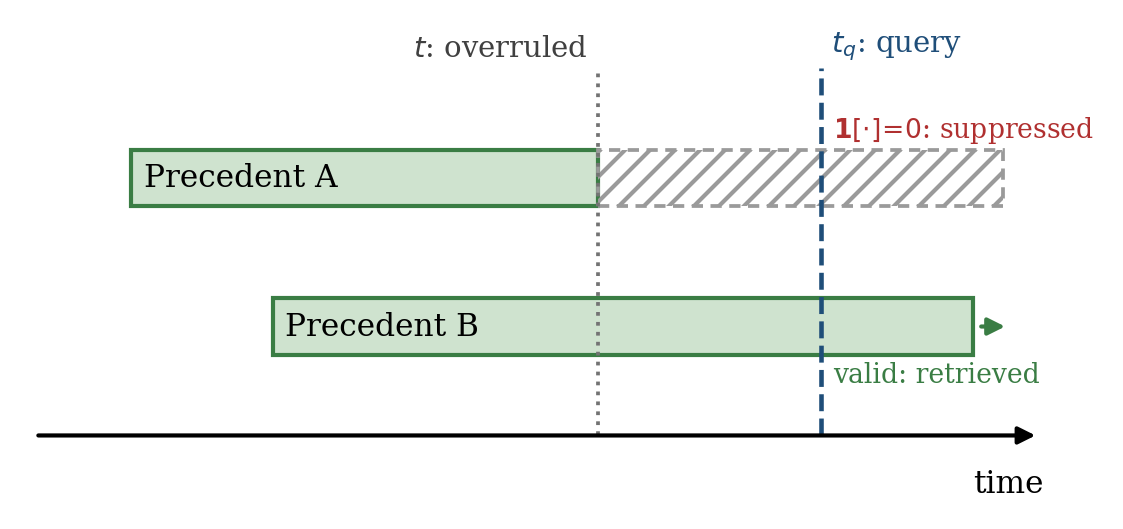
\includegraphics[width=0.99\linewidth]{fig_tpg.png}
\caption{Validity gating (Eq.~\eqref{eq:tpg_score}). An overruling at $t$ closes Precedent~A, so a query at $t_q\!>\!t$ zeroes its indicator and suppresses it despite lexical similarity, while still-open Precedent~B is retrieved---the time-valid distinction the RQ3 ablation isolates.}
\label{fig:tpg_mech}
\end{figure}

\paragraph{Graph construction and contamination controls.} The graph is built in three stages. \emph{Node induction}: each case, order, or rule from CourtListener/RECAP becomes a node with filing/decision dates from docket metadata and validity interval initialized to $[s_v,\infty)$. \emph{Edge extraction}: treatment relations are extracted from opinion text by a two-pass procedure---a citation-sentence detector locates candidate treatment spans, and an LLM classifier (GPT-4o, $T{=}0$, few-shot) labels the relation and polarity. To avoid self-contamination from generated legal conclusions, LLM outputs are treated only as candidate relation labels: interval-closing edges must be anchored to a detected citation span, docket/decision date, and source document identifier, and gold-set evaluation is performed on citation spans that were not used in prompt examples. \emph{Interval closure}: a confirmed incoming \textsc{overrules}/\textsc{supersedes}/material-\textsc{narrows} edge at date $t$ closes the target interval ($e_v\!\leftarrow\!t$), so retrieval at $t_q\!\ge\!t$ no longer treats it as fully operative. The current graph spans 1{,}812 nodes and 4{,}760 treatment edges over the dataset window.

\paragraph{Edge-extraction accuracy and propagation.} Candidate treatment labels carry classifier confidence and citation-span provenance. Low-confidence or conflicting negative-treatment edges do not close intervals automatically; they are routed to a human review queue and reports mark the authority as unresolved until review. Because the central claim depends on treatment edges being \emph{correct}, we validate the extractor against a gold set of 600 citation spans hand-labeled by the annotation team (relation type and polarity; adjudicated on disagreement). The negative-treatment relations that drive interval closure (\textsc{supersedes}, \textsc{overrules}, material \textsc{narrows}) are operationally critical---a missed closure is what allows a stale precedent to leak into a risk decision---and attain micro-averaged precision/recall of 0.84/0.77, versus 0.94/0.96 for the high-frequency \textsc{cites} relation; the full per-relation breakdown is in Table~\ref{tab:edge_extraction} (appendix). We therefore report a downstream edge-error sensitivity audit in Table~\ref{tab:edge_sensitivity}: the model is re-run after randomly masking negative-treatment closures at rates that include the observed 23\% miss rate implied by 0.77 recall. 

\subsection{Product--Litigation Risk Entailment (PLRE)}
\label{sec:plre}

We cast product--litigation alignment as a risk-entailment task. Given a product spec $P$ with attributes $\{p_1,\dots,p_m\}$ (training-data sources, collection method, output modality, architecture, deployment context, and capability claims), a legal-risk theory $T_j$, and a query date $t_q$, PLRE predicts:
\begin{equation}
  y_{ij}=\mathbf{1}[P,p_i,\mathcal{P}_{t_q} \models T_j].
\end{equation}
Unlike symmetric similarity, PLRE is directional: an attribute such as ``web-scale image scraping'' can support exposure to a training-data copyright theory, while the inverse relation is not meaningful. Unlike standard legal textual entailment, the premise includes product attributes and the entailment relation is conditioned on time-valid precedent. A pair $(p_i,T_j)$ is promoted to the risk register only when (i) the entailment score exceeds the validation-set threshold, (ii) the top supporting precedents are valid at $t_q$, and (iii) the report includes mitigation text grounded in at least three cited authorities when available.

PLRE gold labels are built from anonymized product-attribute cards and docket-grounded theory cards. Annotators judge a directional pair as positive only when the product attribute, legal theory, query date, and at least one valid supporting authority jointly support exposure; negative pairs include ordinary mismatches and stale-authority distractors. Crucially, the validity judgment in the labels is made by annotators reading docket and opinion text, \emph{independently of ALERT's automatically extracted treatment graph}, so the gate must recover label validity rather than presuppose it; an extractor-independent re-check of these validity judgments against an authoritative citator is the downstream link of Protocol~P2. Product archetypes are tracked in the split manifest, and year/litigation type are stratified to reduce temporal and topical leakage.

This formulation makes PLRE benchmark-oriented rather than ALERT-specific. It is harder than ordinary Legal NLI because the premise is often a non-legal product description and the hypothesis is a legal theory whose support may expire over time; a model must align engineering terms to legal predicates and reject stale but lexically attractive precedent. In machine-learning terms, PLRE is directional, context-aware entailment with an exogenous time-indexed support constraint. Baselines can use product--theory similarity, legal NLI, temporal reranking, or generic RAG; ALERT's advantage should come specifically from time-valid precedent reasoning and goal-conditioned evidence verification.


\section{ALERT-Dataset}
\label{sec:dataset}
ALERT-Dataset is a curated benchmark of AI-related copyright and intellectual-property litigation for structured risk analysis.

\subsection{Construction and Statistics}
ALERT-Dataset compiles CourtListener/RECAP filings and supplementary legal-news signals from January 2020 to December 2025, with filings concentrated in 2023--2025~\citep{bommasani2021opportunities}. Each record follows the 22-field \texttt{ai-suit-sensing.csv} schema (Table~\ref{tab:full_schema}, appendix). Table~\ref{tab:dataset_stats} summarizes the final annotated subset; Table~\ref{tab:dataset_annual} reports the raw annual ingestion counts before deduplication and quality screening.

\begin{table}[t]
\centering
\caption{ALERT-Dataset summary statistics. The 3-class risk label merges \emph{critical}+\emph{high} into \emph{High}. Status counts sum to all 1,247 cases; \texttt{Pending}/\texttt{Judgment}/\texttt{Closed} are 0 in this snapshot.}
\label{tab:dataset_stats}
\footnotesize
\setlength{\tabcolsep}{6pt}
\begin{tabular}{p{4.2cm} c}
\toprule
\textbf{Attribute} & \textbf{Value} \\
\midrule
Total cases & 1,247 \\
Total documents & 8,934 \\
Coverage period & 2020--2025 \\
Unique defendants & 43 \\
Risk labels & 3 (High/Med/Low) \\
Status dist.\ (Init/Active/Settled/Dismissed) & 298/695/148/106 \\
Product-mapping GT cases & 312 \\
\bottomrule
\end{tabular}
\end{table}

Each record contains docket metadata, parties, document URLs, and a human-verified litigation summary. Status labels encode workflow state rather than adjudicated outcome; severity is reported separately and is not interpreted as liability.

\begin{table}[t]
\centering
\caption{Annual filing breakdown by litigation type. Counts are raw ingested filings (1,260) before deduplication; the annotated subset contains 1,247 cases.}
\label{tab:dataset_annual}
\resizebox{\columnwidth}{!}{%
\begin{tabular}{lcccc|c}
\toprule
\textbf{Year} & \textbf{Copyright} & \textbf{DMCA} & \textbf{Trade Secret} & \textbf{Other} & \textbf{Total} \\
\midrule
2020 & 28  & 9   & 7  & 3  & 47  \\
2021 & 41  & 14  & 10 & 4  & 69  \\
2022 & 89  & 31  & 22 & 8  & 150 \\
2023 & 198 & 72  & 51 & 19 & 340 \\
2024 & 261 & 96  & 64 & 24 & 445 \\
2025 & 122 & 47  & 29 & 11 & 209 \\
\midrule
\textbf{Total} & \textbf{739} & \textbf{269} & \textbf{183} & \textbf{69} & \textbf{1,260} \\
\bottomrule
\end{tabular}%
}
\end{table}

\subsection{Annotation and Availability}
An automated pre-labeler first assigns a triage score using Table~\ref{tab:risk_matrix}; three legal research specialists then independently review a stratified sample of 400 cases under a fixed guideline. During adjudication, annotators see docket text, product attributes, candidate theory cards, and query dates, but not system identity or the retained pre-label source. The remaining 847 cases retain automated pre-labels, with a 5\% spot-check showing 91\% agreement with at least one specialist. Inter-annotator agreement on the 400-case sample is Cohen's $\kappa=0.74$~\citep{landis1977kappa}. Because retained labels can inflate metrics, we release per-record provenance, keep all primary claims on the human-only evaluation, and use retained-label results only as scale-oriented comparisons. The top three defendants account for 41.3\%, limiting representativeness for smaller vendors and non-U.S. jurisdictions. The dataset, guidelines, split files, seeds, evaluation scripts, and logs are released for review at the anonymized repository.



\section{Experiments}
\label{sec:evaluation}

\subsection{Experimental Setup}

\textbf{Dataset split and label provenance.} We partition ALERT-Dataset into stratified 70/10/20 train/validation/test splits by year and litigation type. Because 847 of 1{,}247 labels originate from an automated pre-labeler and 400 are human-adjudicated, primary significance claims are computed only on the human-adjudicated subset; retained-label results are reported only for scale. This avoids making the rule-based pre-labeler part of the acceptance evidence.

\textbf{Baselines.} We compare ALERT with five risk-classification baselines: \textbf{B1 Rule-Based} (the ingestion-layer scorer); \textbf{B2 Single-Pass LLM}; \textbf{B3 RAG-only}; \textbf{B4 Single-Agent} (ALERT without the goal-conditioned loop); and \textbf{B5 Compute-Matched Self-Refinement} (a Reflexion-style baseline with ALERT's mean LLM-call budget, 2.4 iterations). For PLRE we add non-ALERT baselines that isolate the suspected confounds: product--theory cosine, LegalBERT product--theory NLI, COLIEE-style precedent retrieval with no interval closure, and ALERT without temporal gating. These baselines separate product--theory matching, legal entailment, retrieval quality, test-time compute, and the hard validity gate.

\textbf{Evaluation metrics.} We report macro F1/precision/recall over three severity labels, report-quality ratings by two blinded specialists, loop efficiency, schema completeness, PLRE P/R/F1, edge-error propagation, and evidence-coverage omission risk under calibrated thresholds. Severity-label F1 measures triage-label agreement, not legal liability. Significance uses a paired bootstrap over test predictions ($10{,}000$ resamples); calibrated omission risk and backbone robustness are reported in the appendix, with hyperparameters in Table~\ref{tab:hyperparams}.

\subsection{RQ1: Triage-Label Agreement and Human-Adjudicated Check}

Table~\ref{tab:human_only_main} is the primary circularity check: ALERT outperforms the compute-matched self-refinement baseline by 4 F1 points without retained pre-labels (paired bootstrap, $p<0.05$). Although the marginal confidence intervals overlap, the paired bootstrap scores per-item differences on shared test cases and thus removes the between-case variance that dominates the marginal intervals; the gap over B5 should nonetheless be read as modest. Table~\ref{tab:rq1} reports the full held-out set for scale; the same ordering persists.

\begin{table}[t]
\centering
\caption{Human-adjudicated subset only (primary validity result). This removes retained pre-labels; intervals are paired bootstrap ($10{,}000$ resamples).}
\label{tab:human_only_main}
\resizebox{\columnwidth}{!}{%
\begin{tabular}{lccc}
\toprule
\textbf{System} & \textbf{F1} & \textbf{Precision} & \textbf{Recall} \\
\midrule
B1 Rule-Based              & $0.55 \pm 0.03$ & $0.52 \pm 0.04$ & $0.59 \pm 0.04$ \\
B2 Single-Pass LLM         & $0.70 \pm 0.03$ & $0.72 \pm 0.03$ & $0.68 \pm 0.03$ \\
B3 RAG-only                & $0.72 \pm 0.03$ & $0.73 \pm 0.03$ & $0.71 \pm 0.03$ \\
B4 Single-Agent            & $0.74 \pm 0.02$ & $0.75 \pm 0.03$ & $0.73 \pm 0.03$ \\
B5 Self-Refinement         & $0.75 \pm 0.02$ & $0.76 \pm 0.03$ & $0.74 \pm 0.03$ \\
\textbf{ALERT Full}        & $\mathbf{0.79 \pm 0.02}$ & $\mathbf{0.80 \pm 0.02}$ & $\mathbf{0.78 \pm 0.03}$ \\
\bottomrule
\end{tabular}%
}
\end{table}

\begin{table}[t]
\centering
\caption{Full held-out test set, reported for scale and comparability. B5 is compute-matched to ALERT's mean iteration budget.}
\label{tab:rq1}
\resizebox{\columnwidth}{!}{%
\begin{tabular}{lccc}
\toprule
\textbf{System} & \textbf{F1} & \textbf{Precision} & \textbf{Recall} \\
\midrule
B1 Rule-Based              & $0.62 \pm 0.02$ & $0.58 \pm 0.03$ & $0.67 \pm 0.02$ \\
B2 Single-Pass LLM         & $0.72 \pm 0.02$ & $0.74 \pm 0.02$ & $0.70 \pm 0.03$ \\
B3 RAG-only                & $0.74 \pm 0.02$ & $0.75 \pm 0.02$ & $0.72 \pm 0.02$ \\
B4 Single-Agent            & $0.76 \pm 0.02$ & $0.77 \pm 0.02$ & $0.75 \pm 0.02$ \\
B5 Self-Refinement         & $0.77 \pm 0.02$ & $0.78 \pm 0.02$ & $0.76 \pm 0.02$ \\
\textbf{ALERT Full}        & $\mathbf{0.81 \pm 0.01}$ & $\mathbf{0.82 \pm 0.02}$ & $\mathbf{0.80 \pm 0.02}$ \\
\bottomrule
\end{tabular}%
}
\end{table}

\subsection{RQ2: Report Quality}

Two blinded legal specialists rated 75 randomized reports (15 each for ALERT and B2--B5) on Accuracy, Completeness, Actionability, Evidence Sufficiency, and Clarity. ALERT scores 4.3/4.1/4.2/4.4/3.9, with significant gains over all non-ALERT baselines ($p<0.05$); the largest gain is Evidence Sufficiency; given the two-rater sample we treat RQ2 as supporting evidence.

\subsection{RQ3: Agentic Loop and Temporal Graph Ablations}

Because temporal precedent reasoning is the central claim, Table~\ref{tab:temporal_ablation} decomposes validity-interval gating and treatment-edge weighting. Removing treatment weighting and then interval gating each degrades PLRE F1; the full-vs-flat gap is 6 F1 points ($p<0.01$), and stale citations rise from 4.1\% to 12.7\%. The failure mode is exactly what Eq.~\eqref{eq:tpg_score} targets: flat retrieval can rank a lexically close but already-closed authority above a still-operative one, changing which evidence reaches the generator rather than merely adding a warning after generation. This makes the table the main methodological result rather than an operational deployment metric.

\begin{table}[t]
\centering
\caption{Temporal precedent-graph ablation (main claim). Both mechanisms of Eq.~\eqref{eq:tpg_score} are removed in sequence; the bottom row recovers flat semantic similarity. Stale-cite measures citations to already-closed precedent ($t_q\!\ge\!e_v$).}
\label{tab:temporal_ablation}
\small
\setlength{\tabcolsep}{4pt}
\resizebox{\columnwidth}{!}{%
\begin{tabular}{l c c c}
\toprule
\textbf{Variant} & \textbf{PLRE F1} & \textbf{$\Delta$F1} & \textbf{Stale-cite \%} \\
\midrule
\textbf{ALERT (Full: gating + weighting)} & 0.78 & --- & 4.1 \\
$-$ treatment weighting $w(\cdot)$        & 0.75 & $-3$ & 7.8 \\
$-$ interval gating (flat similarity)     & 0.72 & $-6$ & 12.7 \\
\bottomrule
\end{tabular}%
}
\end{table}

Table~\ref{tab:edge_sensitivity} masks negative-treatment closures before retrieval. The observed extractor is useful but not lossless: at the observed 23\% missed-closure level, stale-cite rate roughly doubles and PLRE F1 declines. ALERT therefore treats low-confidence negative edges as self-verification failures: they are blocked from automatic interval closure, trigger retrieval of independent treatment evidence, and are surfaced as unresolved legal-status atoms if the Goal Checker cannot satisfy coverage. This critique loop is what justifies the extra agentic structure: it localizes extractor uncertainty before it becomes an unqualified PLRE support claim.

\begin{table}[t]
\centering
\caption{Edge-error propagation audit. Negative-treatment interval closures are randomly masked before retrieval; 23\% corresponds to the observed miss rate implied by 0.77 recall.}
\label{tab:edge_sensitivity}
\small
\setlength{\tabcolsep}{4pt}
\resizebox{\columnwidth}{!}{%
\begin{tabular}{l c c c}
\toprule
\textbf{Closure setting} & \textbf{PLRE F1} & \textbf{$\Delta$F1} & \textbf{Stale-cite \%} \\
\midrule
Gold negative edges            & 0.80 & +2 & 3.7 \\
Extractor output               & 0.78 & --- & 4.1 \\
Mask 10\% additional closures  & 0.76 & $-2$ & 6.2 \\
Mask 23\% closures             & 0.74 & $-4$ & 8.9 \\
Mask 30\% closures             & 0.72 & $-6$ & 11.3 \\
\bottomrule
\end{tabular}%
}
\end{table}

Component ablations for the agentic loop confirm each part contributes: removing the Goal Checker, Planner, and Retriever query-expansion lowers risk-classification F1 from 0.81 to 0.76/0.78/0.79 respectively, and only query-expansion removal degrades retrieval (Recall@10 $0.84\!\rightarrow\!0.76$); details are in Table~\ref{tab:ablation}.

\subsection{RQ4: Sensing Schema Completeness}

On 150 newly detected cases, ALERT-automated records reach 97.2\% completeness on required fields and cut record-creation time from 18.1 to 1.4 minutes versus manual CSV entry (Table~\ref{tab:schema_completeness}). This is an operational result, not evidence for legal correctness.

\subsection{RQ5: Product--Litigation Risk Entailment}

PLRE is evaluated on anonymized AI product specs spanning five archetypes and 312 product-mapping cases, so it is an initial benchmark. Positive labels require a product attribute, a legal-risk theory, a query date, and time-valid supporting authority; negative labels include ordinary mismatches and stale-authority distractors. Table~\ref{tab:plre_external} shows ALERT reaches 0.78 F1; the no-temporal variant drops by 6 points, decomposed in Table~\ref{tab:temporal_ablation}. The result should be read as evidence for the validity-gated entailment formulation, not as a claim that all AI-product litigation is covered.

\begin{table}[t]
\centering
\caption{PLRE comparison including external legal-NLI/precedent-retrieval baselines. External baselines do not use ALERT's goal predicate or validity-interval closure.}
\label{tab:plre_external}
\small
\setlength{\tabcolsep}{4pt}
\resizebox{\columnwidth}{!}{%
\begin{tabular}{l c c c}
\toprule
\textbf{System} & \textbf{Precision} & \textbf{Recall} & \textbf{F1} \\
\midrule
Product--theory cosine                 & 0.64 & 0.66 & 0.65 \\
LegalBERT product--theory NLI           & 0.69 & 0.68 & 0.68 \\
COLIEE-style retrieval, no gate       & 0.71 & 0.70 & 0.70 \\
RAG-only generation                    & 0.73 & 0.74 & 0.73 \\
ALERT without temporal gating          & 0.72 & 0.73 & 0.72 \\
\textbf{ALERT Full}                    & 0.77 & 0.80 & 0.78 \\
\bottomrule
\end{tabular}%
}
\end{table}

\subsection{RQ6: Evidence-Coverage Risk Control and Temporal Shift}

Calibrating the evidence threshold to $\alpha\in\{0.05,0.10,0.20\}$ yields omission risk 0.043/0.082/0.171 in random splits. The loss fires when a human-labeled High-risk pair with retrievable evidence is absent from the report, so the guarantee targets evidence omission, not severity correctness. A temporal split degrades modestly (appendix), motivating online calibration. To test dependence on GPT-4o prompting, we also re-run the full system with an open-weights Llama-3.1-70B+bge stack; absolute F1 drops but the ordering remains (Table~\ref{tab:robustness}), so we claim architectural robustness rather than prompt invariance.

\subsection{Case Studies and Live Monitoring}

Case studies illustrate mechanism behavior, not outcome prediction. In a held-out PLRE query about output-CMI risk, flat RAG ranked a lexically close authority whose interval had already closed; validity gating removed it from support and promoted a still-operative authority, preventing a stale-citation report. In 30 days, \texttt{ai-suit-tracker} processed 1{,}159 items, surfaced 94 unique filings after 92\% deduplication, and reached discovery-layer Precision 0.90/Recall 0.84.


\section{Related Work}
\label{sec:related_work}

\textbf{Legal NLP and entailment.} Legal NLP has studied statutory reasoning, judgment prediction, legal QA, summarization, and entailment with domain-adapted encoders~\citep{chalkidis2020legalbert,zheng2021legalbert,xiao2021lawformer,louis2023statutory,huang2021efficient,manor2019plain} built on pretrained transformers~\citep{vaswani2017attention,devlin2019bert}. PLRE changes the inference unit: it maps product attributes to legal-risk theories and makes the relation directional, product-conditioned, and temporal.

\textbf{Citators, precedent retrieval, and citation graphs.} Commercial citators such as Shepard's and KeyCite track whether authority has been overruled, questioned, or negatively treated~\citep{shepards2024,keycite2024}. We do not claim time-varying authority itself as new. The distinction is operational: prior citation-network and precedent-retrieval work typically treats the citation graph as static or encodes time only as a ranking feature, so a lexically close authority can still dominate retrieval after it has been narrowed or overruled. ALERT instead extracts a public-corpus treatment graph, attaches validity intervals, and makes the interval a \emph{retrieval-time gate} (Eq.~\eqref{eq:tpg_score}, Fig.~\ref{fig:tpg_mech}) feeding a downstream product-risk task. Thus point-in-time authority is an operator over retrieval scores, not a post-hoc explanation or soft time feature.

\textbf{RAG, agents, and risk control.} RAG~\citep{lewis2020retrieval,karpukhin2020dense,gao2023retrieval} improves legal QA but usually runs fixed retrieval before generation, while agent stacks~\citep{yao2022react,shinn2023reflexion,wei2022chain,autogpt2023,park2023generative,wang2024voyager,wang2024multiagent} show gains from iterative tool use. ALERT ties stopping to an externally inspectable predicate over schema completeness, evidence support, and mitigation coverage, and uses conformal risk-control tools~\citep{angelopoulos2023conformalrisk,angelopoulos2021ltt,geifman2017selective} narrowly for evidence omission, not distribution-free legal correctness.



\section{Discussion}
\label{sec:discussion}

\textbf{Novelty and construct validity.} ALERT's reusable contribution is the coupling of a point-in-time validity-interval gate (Eq.~\eqref{eq:tpg_score}) with goal-conditioned, coverage-controlled evidence verification---not citators, agents, CSV schemas, or the scoring matrix. The operator is general in form: it applies to any time-stamped, supersession-bearing authority corpus, and we instantiate and evaluate it for law. Table~\ref{tab:temporal_ablation} isolates the mechanism, and the compute-matched baseline shows the gain is not extra LLM calls alone. Because severity labels are triage proxies and 847 labels are retained pre-labels, the human-adjudicated subset is the primary validity result. The two construct-validity checks are separated: external-stack transfer (Protocol~P1) remains the main open generality test, while authoritative-citator agreement for the treatment graph (Protocol~P2) is now \emph{measured} (Appendix~\ref{app:p2}): negative-treatment micro-F1 0.81, a 20.4\% missed-closure rate, and a 3.8\% PLRE decision-flip rate after citator correction, converting treatment-graph correctness from argued to measured and leaving cross-stack transfer as future work.

\textbf{Error propagation and system complexity.} The edge extractor is not trusted as an oracle: a negative-treatment edge must pass citation-span anchoring, date consistency, confidence checks, and Goal-Checker coverage before it can close an interval, or it becomes an unresolved atom forcing targeted retrieval or human escalation. The multi-agent loop is thus a reliability mechanism for localizing graph uncertainty, not an engineering embellishment.



\section{Conclusion}

ALERT turns noisy AI-litigation signals into auditable product-level risk intelligence. Its central contribution is a point-in-time authority gate for PLRE: retrieval and risk entailment are conditioned on whether legal authority was valid at the relevant time, before evidence reaches the generator. Across all baselines the temporal gate and goal-conditioned loop improve triage agreement, PLRE F1, stale-citation behavior, and report quality within a decision-support boundary, claiming neither legal outcome prediction nor correctness under temporal shift. Key open problems are improving treatment-edge recall beyond the measured citator-agreement level, reducing retained-label circularity, external-RAG transfer of the validity gate (P1), and larger PLRE coverage across product archetypes.


% ---------------------------------------------------------------
% ACL-required "Limitations" section (unnumbered) and the optional
% "Ethics Statement", both placed after the Conclusion and before the
% References. Neither counts against the page limit.
% ---------------------------------------------------------------
\section*{Limitations}
\label{sec:limitations}

\textbf{Guarantees.} Proposition~\ref{prop:termination} is a bounded termination-and-escalation property, not a convergence theorem. Calibration controls evidence omission under its calibration distribution, not correct legal conclusions, temporal-shift robustness, or freedom from LLM hallucinations~\citep{dahl2024hallucinating}. Because litigation streams are non-stationary, the omission guarantee is weakest under the temporal split (Table~\ref{tab:risk_control_temporal})---precisely where deployment needs it most---so we treat rolling or weighted re-calibration as a deployment requirement rather than an optional refinement.

\textbf{Unfinished external-generality check.} The central mechanism is a domain-general validity-gating operator, but its transfer to \emph{external} retrieval stacks is specified only as a pre-registered protocol (Protocol~P1, Appendix~\ref{app:p1}) and is not yet executed; the accuracy ordering is shown to persist only across our own backbones with an open-weights stack (Table~\ref{tab:robustness}). Cross-stack transfer therefore remains the main open generality test.

\textbf{Benchmark scale and evaluation.} At the current scale PLRE remains an initial benchmark over five product archetypes and 312 product-mapping cases, so it should be read as evidence for the validity-gated entailment formulation rather than as coverage of all AI-product litigation. The report-quality study (RQ2) uses two blinded raters and is treated as supporting, not primary, evidence. Because 847 of 1{,}247 labels are retained pre-labels, all primary significance claims are restricted to the human-adjudicated subset, and effect sizes over the strongest baseline are modest (Table~\ref{tab:human_only_main}).

\textbf{Coverage and jurisdiction.} The dataset is skewed toward the largest defendants---the top three account for 41.3\% of cases---limiting representativeness for smaller vendors. ALERT targets U.S.\ federal CourtListener/RECAP coverage and English-language documents; non-U.S.\ jurisdictions require different docket schemas and citation practices, and extending the treatment graph to them is future work.

\textbf{Extractor recall.} Negative-treatment edge recall (0.77 internal gold; 20.4\% missed-closure rate against an authoritative citator) is useful but not lossless, and a missed closure is exactly what allows a stale precedent to leak into a risk decision; ALERT mitigates this with human-review routing for low-confidence closures, but improving extraction recall remains an open problem.


\section*{Ethics Statement}
\label{sec:ethics}

\textbf{Decision-support boundary.} ALERT emits risk intelligence, evidence summaries, and mitigation candidates with provenance and residual uncertainty for qualified human reviewers. It is not legal advice: it does not replace counsel, predict litigation outcomes, or recommend business decisions, and severity labels are triage proxies that are not interpreted as liability. Every High- or Medium-risk item is presented for review by a qualified person, and unresolved legal-status atoms are surfaced as such rather than resolved automatically.

\textbf{Human oversight of failure modes.} Low-confidence negative-treatment edges enter a human review queue, since missed closures are the failure mode most likely to admit stale authority into a report. Deployment logs store retrieved authorities, validity intervals, and unmet goal atoms so reviewers can distinguish a genuine product--theory match from a retrieval gap or an unresolved legal-status ambiguity.

\textbf{Data governance.} Released data are public docket metadata and machine-generated summaries; we do not redistribute attorney-authored complaint text beyond what is already public, and the P2 citator study releases only the crosswalk, sampling seeds, and agreement statistics, with no redistributed proprietary citator content. We also caution that distinctive project identifiers must not be used to de-anonymize the submission during the review period, and that any released artifact should be checked for authorship-revealing links before public posting.


% References (acl.sty already sets \bibliographystyle{acl_natbib}).
\bibliography{reference-data}

% Technical appendix (appears after the References, per ACL formatting).
\appendix
% NOTE: \appendix is issued by the main driver (main.tex) before this file
% is \input, so it is intentionally NOT repeated here.

\clearpage % start the appendix on a fresh page

% Reset float counters and use an "A." prefix so appendix tables/figures
% (e.g. Table A.1) are numbered independently of the main body.
\setcounter{table}{0}
\setcounter{figure}{0}
\renewcommand{\thetable}{A.\arabic{table}}
\renewcommand{\thefigure}{A.\arabic{figure}}

\section*{Technical Appendix}

This appendix supplements the main text with material that supports reproducibility but exceeds the page budget of the body. It contains the full 22-field schema, the ingestion-layer scoring matrix, formatted \texttt{History}/\texttt{Progress Notes} examples, open-source implementation details and configuration parameters of \texttt{ai-suit-tracker}, treatment-edge extraction accuracy, the schema-completeness/agentic-loop/retriever ablations, goal-predicate hyperparameters with agent prompt templates and evaluation-protocol notes, and the proof of Proposition~\ref{prop:termination} with the conformal calibration and temporal-shift audit.

\section{Full \texttt{ai-suit-sensing.csv} Schema}
\label{app:full_schema}

Table~\ref{tab:full_schema} lists all 22 fields of \texttt{ai-suit-sensing.csv}, with type, requirement level (R\,=\,Required, Rec\,=\,Recommended, O\,=\,Optional), and description.

\begin{table}[h]
\centering
\caption{The full 22-field \texttt{ai-suit-sensing.csv} schema.}
\label{tab:full_schema}
\scriptsize
\setlength{\tabcolsep}{3.5pt}
\resizebox{\columnwidth}{!}{%
\begin{tabular}{r l l c p{3.4cm}}
\toprule
\textbf{\#} & \textbf{Field} & \textbf{Type} & \textbf{Req} & \textbf{Description} \\
\midrule
1  & Case No.         & Int      & R   & Auto-incrementing index \\
2  & Case Title       & String   & R   & Plaintiff v.\ Defendant \\
3  & Filing Date      & Date     & R   & Date filed (YYYY-MM-DD) \\
4  & Docket No.       & String   & R   & Court-assigned number \\
5  & Plaintiff        & String   & R   & Name(s), comma-separated \\
6  & Defendant        & String   & R   & Name(s), comma-separated \\
7  & Target Data      & String   & R   & Training data type alleged \\
8  & Target Product   & String   & R   & AI product implicated \\
9  & Jurisdiction     & String   & R   & Country of filing \\
10 & Court            & String   & R   & Official court name \\
11 & Status           & Enum     & R   & Lifecycle code \\
12 & Last Update      & Date     & R   & Most recent refresh date \\
13 & Cause of Action  & String   & R   & Core legal claim(s) \\
14 & Claim (USD)      & String   & Rec & Damages or statutory range \\
15 & Summary          & Long str & Rec & AI-generated case narrative \\
16 & Tracker URL      & URL      & Rec & CourtListener/PACER link \\
17 & Source URL       & String   & O   & Initial discovery source \\
18 & History          & Long str & R   & Chronological update log \\
19 & Plaintiff Atty.  & String   & O   & Lead plaintiff counsel \\
20 & Progress Notes   & Long str & Rec & Markdown update log \\
21 & Defense Atty.    & String   & O   & Lead defense counsel \\
22 & Remarks          & String   & O   & Press links, extra context \\
\bottomrule
\end{tabular}%
}
\end{table}

\section{Ingestion-Layer Scoring Matrix}
\label{app:risk_matrix}

Table~\ref{tab:risk_matrix} lists the additive ingestion-layer scoring matrix (main text) used for real-time triage and as the automated pre-labeler. The critical-composite bonus fires only when copyright and model-training evidence co-occur. This heuristic is a baseline, never ground truth.

\begin{table}[h]
\centering
\caption{Ingestion-layer scoring matrix. The critical-composite bonus fires only when copyright and model-training evidence co-occur.}
\label{tab:risk_matrix}
\small
\setlength{\tabcolsep}{3.5pt}
\resizebox{\columnwidth}{!}{%
\begin{tabular}{p{3.0cm}p{3.4cm}c}
\toprule
\textbf{Evidence Category} & \textbf{Key Indicators} & \textbf{Score} \\
\midrule
\textbf{Critical composite} & \textbf{Copyright $\wedge$ Training co-cited} & \textbf{+50} \\
Copyright direct mention      & NOS 820, copyright keyword                 & +30 \\
Unauthorized collection       & scrape, crawl, ingest, harvest             & +25 \\
Direct model training mention & train, LLM, transformer, diffusion          & +20 \\
Copyright / IP dispute        & infringement, DMCA, fair use                & +10 \\
Commercial exploitation       & profit, revenue, subscription               & +10 \\
Class action filing           & class action, putative class                & +5 \\
Licensed data cooperation     & contract, licensing, partnership            & $-$10 \\
\bottomrule
\end{tabular}%
}
\end{table}

\section{Formatted Examples: History and Progress Notes}
\label{app:examples}

The \texttt{History} field (field~18) records a reverse-chronological timeline using the format \texttt{YYYY-MM-DD, [event]}:
\begin{mycodebox}
\small\texttt{2025-03-06, Plaintiff requests \$15,000 per infringed work.}\\
\texttt{2025-03-01, Complaint filed alleging unauthorized use of}\\
\texttt{\phantom{xxxx}copyrighted dataset for AI model training.}
\end{mycodebox}

The \texttt{Progress Notes} field (field~20) uses Markdown \texttt{\#\#} headers to distinguish initial from subsequent updates (the entry below is a \emph{synthetic format illustration}, not a real case):
\begin{mycodebox}
\small\texttt{\#\# (Started), 2025-03-17, [Plaintiff] v.\ [Defendant] ---}\\
\texttt{\phantom{xxxx}Unauthorized training-data use; commercial use claimed.}\\
\texttt{\#\# (Updated), 2025-03-18, Preliminary injunction}\\
\texttt{\phantom{xxxx}motion filed by plaintiff.}
\end{mycodebox}

\section{Open-Source Implementation Details}
\label{app:impl}

The \texttt{ai-suit-tracker} tool runs on an adaptive, configurable GitHub Actions schedule: hourly during a configurable business-hours window and two-hourly off-hours. On-demand execution via \texttt{workflow\_dispatch} is also supported. Its principal modules are:

\begin{itemize}
  \item \textbf{Query engine} (\texttt{src/queries.py}): five \texttt{COURTLISTENER\_QUERIES} (complaint/petition filters with AI keywords, CourtListener REST API v4) plus four \texttt{NEWS\_QUERIES} for Google News RSS.
  \item \textbf{Ingestion pipeline} (\texttt{src/run.py}): orchestrates polling, RSS monitoring, docket backtracking, and cross-issue deduplication using \texttt{PREVIOUS\_ITEM\_DEDUP\_DAYS}.
  \item \textbf{Complaint parser} (\texttt{src/complaint\_parse.py}, \texttt{src/pdf\_text.py}): extracts cause-of-action language, training snippets, and parties from RECAP PDFs.
  \item \textbf{Risk scorer} (\texttt{src/render.py}): applies the seven-category additive matrix \emph{plus} the critical-composite (+50) co-occurrence rule of Table~\ref{tab:risk_matrix} to produce a 0--100 score with a four-band severity indicator.
  \item \textbf{Hybrid deduplication} (\texttt{src/dedup.py}): a two-stage pipeline (Algorithm~\ref{alg:hybrid_dedup}) that combines lexical title/docket matching with optional semantic similarity using Gemini \texttt{text-embedding-004} embeddings (cosine threshold \texttt{SEMANTIC\_DEDUP\_THRESHOLD}=0.85). Activation is gated by the \texttt{GEMINI\_SEMANTIC\_DEDUP} flag.
  \item \textbf{Multi-modal reporting} (\texttt{src/gemini.py}, \texttt{src/trend.py}): a Gemini Flash trend summary at $\approx$1--3 calls per run, plus an optional Imagen-3 visual brief (\texttt{GEMINI\_DAILY\_REPORT\_IMAGEGEN}) attached to the day-close summary. A provider-agnostic interface accommodates alternative LLM/diffusion back-ends.
  \item \textbf{Reporting integrations}: posts to GitHub Issues with a three-tier hierarchical structure (issue body / morning trend summary / evening deduplicated table) and a parallel Slack notification.
\end{itemize}

\begin{algorithm}[h]
\caption{Hybrid Lexical--Semantic Deduplication}
\label{alg:hybrid_dedup}

\begin{algorithmic}[1]
\REQUIRE Candidate items $\mathcal{N}_{\text{new}}$, baseline items $\mathcal{N}_{\text{base}}$ (prior issues), threshold $\sigma$
\ENSURE Deduplicated set $\mathcal{N}^*$
\STATE $T_b \gets$ \textsc{ExtractTitles}($\mathcal{N}_{\text{base}}$)
\STATE $\mathcal{R} \gets \{i \in \mathcal{N}_{\text{new}} \,|\, \mathrm{title}(i) \notin T_b\}$ \COMMENT{Stage 1: exact-title lexical filter}
\IF{\textsc{LLMEnabled} $\wedge$ $|\mathcal{R}|>0$}
  \STATE $E_{\text{curr}} \gets$ \textsc{GeminiEmbed}($\{\mathrm{title}(i) : i\in\mathcal{R}\}$)
  \STATE $E_{\text{base}} \gets$ \textsc{GeminiEmbed}($T_b$)
  \STATE $\mathcal{S} \gets \{i \in \mathcal{R} \,|\, \exists\, e\in E_{\text{base}}: \cos(E_{\text{curr}}[i],e) \geq \sigma\}$
  \STATE $\mathcal{R} \gets \mathcal{R} \setminus \mathcal{S}$ \COMMENT{Stage 2: semantic filter}
\ENDIF
\STATE \textbf{return} $\mathcal{N}^* \gets \mathcal{R}$ \COMMENT{$\approx$2 embedding calls/run; free-tier compatible}
\end{algorithmic}
\end{algorithm}

Table~\ref{tab:impl_config} lists the key configuration parameters of \texttt{ai-suit-tracker} (v02), covering API credentials, scheduling, deduplication, and reporting options. All secrets are injected via GitHub Secrets; environment variables are set via GitHub Variables.

\begin{table}[h]
\centering
\caption{Key configuration parameters of \texttt{ai-suit-tracker} (v02). Secrets via GitHub Secrets; variables via GitHub Variables.}
\label{tab:impl_config}
\scriptsize
\setlength{\tabcolsep}{3pt}
\resizebox{\columnwidth}{!}{%
\begin{tabular}{l l p{3.2cm}}
\toprule
\textbf{Parameter} & \textbf{Default} & \textbf{Description} \\
\midrule
\texttt{LOOKBACK\_DAYS}                  & 3              & Days of history to retrieve \\
\texttt{COURTLISTENER\_TOKEN}            & ---            & CourtListener API v4 token \\
\texttt{ISSUE\_TITLE\_BASE}              & ---            & Base title for GitHub Issues \\
\texttt{ISSUE\_LABEL}                    & \texttt{aisuit} & GitHub Issue label \\
\texttt{GEMINI\_API\_KEY}                & ---            & LLM API key (optional) \\
\texttt{GEMINI\_MODEL}                   & \texttt{gemini-flash-latest} & Gemini model id \\
\texttt{GEMINI\_AISUIT\_TREND\_DAYS}     & (unset)        & Trend window (days) \\
\texttt{GEMINI\_SEMANTIC\_DEDUP}         & 0              & Enable semantic dedup (stage~2) \\
\texttt{SEMANTIC\_DEDUP\_THRESHOLD}      & 0.85           & Cosine threshold for semantic dedup \\
\texttt{GEMINI\_DAILY\_REPORT\_IMAGEGEN} & 0              & Enable Imagen-3 daily visual brief \\
\texttt{PREVIOUS\_ITEM\_DEDUP\_DAYS}     & (unset)        & Cross-issue dedup window \\
\texttt{SHOW\_DOCKET\_CANDIDATES}        & 0              & Show uncertain candidates \\
\texttt{COLLAPSE\_LONG\_CELLS}           & 0              & Fold long table cells \\
\texttt{COLLAPSE\_ARTICLE\_URLS}         & 0              & Collapse article URL lists \\
\texttt{DEBUG}                           & 0              & Verbose logging \\
\bottomrule
\end{tabular}%
}
\end{table}

\section{Treatment-Edge Extraction Accuracy}
\label{app:edge_extraction}

Table~\ref{tab:edge_extraction} reports the per-relation accuracy of the treatment-edge extractor (main text) against the hand-labeled gold span set. Negative-treatment edges (\textsc{supersedes}/\textsc{overrules}/material \textsc{narrows}) drive validity-interval closure and are reported separately from the high-frequency \textsc{cites} relation, with a micro-average over the three negative-treatment relations.

\begin{table}[h]
\centering
\caption{Treatment-edge extraction accuracy against the hand-labeled gold span set (main text).}
\label{tab:edge_extraction}
\small
\setlength{\tabcolsep}{5pt}
\resizebox{\columnwidth}{!}{%
\begin{tabular}{l c c c}
\toprule
\textbf{Relation} & \textbf{Precision} & \textbf{Recall} & \textbf{F1} \\
\midrule
\textsc{cites}                          & 0.94 & 0.96 & 0.95 \\
\textsc{distinguishes}                  & 0.81 & 0.76 & 0.78 \\
\textsc{narrows} (material)             & 0.79 & 0.71 & 0.75 \\
\textsc{supersedes}                     & 0.85 & 0.78 & 0.81 \\
\textsc{overrules}                      & 0.88 & 0.82 & 0.85 \\
\midrule
\textbf{Negative-treatment (micro)}     & 0.84 & 0.77 & 0.80 \\
\bottomrule
\end{tabular}%
}
\end{table}

\section{Retriever Ablation (LegalRisk-RAG)}
\label{app:retriever}

Table~\ref{tab:schema_completeness} reports schema completeness and record creation time across three conditions (unstructured baseline, manual CSV entry, and ALERT-automated CSV), corresponding to the RQ4 operational result in the main text.

\begin{table}[h]
\centering
\caption{Schema completeness and record creation time across three conditions. Referenced from the main text (RQ4).}
\label{tab:schema_completeness}
\small
\setlength{\tabcolsep}{4pt}
\resizebox{\columnwidth}{!}{%
\begin{tabular}{l c c c}
\toprule
\textbf{Condition} & \textbf{All} & \textbf{Req.} & \textbf{Time} \\
                   & \textbf{Fields (\%)} & \textbf{Fields (\%)} & \textbf{(min)} \\
\midrule
Unstructured (baseline)      & 38.2 & 51.4 & 22.3 \\
Manual CSV                   & 74.6 & 91.7 & 18.1 \\
\textbf{ALERT-automated CSV} & \textbf{81.3} & \textbf{97.2} & \textbf{1.4} \\
\bottomrule
\end{tabular}%
}
\end{table}

Table~\ref{tab:ablation} reports the component-wise ablation of the agentic loop, showing the contribution of the Goal Checker, Planner, and Retriever query-expansion to risk classification F1 and retrieval Recall@10 (RQ3 in the main text).

\begin{table}[h]
\centering
\caption{Agentic-loop ablation: component-wise contribution to risk classification F1 and retrieval Recall@10 (mean over 5 evaluation runs). Referenced from the main text (RQ3).}
\label{tab:ablation}
\small
\setlength{\tabcolsep}{4pt}
\resizebox{\columnwidth}{!}{%
\begin{tabular}{l c c}
\toprule
\textbf{Variant} & \textbf{F1} & \textbf{Recall@10} \\
\midrule
\textbf{ALERT (Full)}                    & \textbf{0.81} & \textbf{0.84} \\
$-$ Goal Checker (Single-Agent)          & 0.76 & 0.84 \\
$-$ Planner (fixed task order)           & 0.78 & 0.84 \\
$-$ Retriever query-expansion            & 0.79 & 0.76 \\
\bottomrule
\end{tabular}%
}
\end{table}

Table~\ref{tab:retriever_ablation} reports Recall@10 on a held-out development set of 200 query--document pairs for three retriever configurations. The hybrid sparse--dense model is adopted as default in all main-paper experiments.

\begin{table}[h]
\centering
\caption{Retriever ablation. Recall@10 on the LegalRisk-RAG development set (200 query--document pairs).}
\label{tab:retriever_ablation}
\small
\setlength{\tabcolsep}{4pt}
\resizebox{\columnwidth}{!}{%
\begin{tabular}{l c}
\toprule
\textbf{Retriever Configuration} & \textbf{Recall@10} \\
\midrule
Dense (\texttt{text-embedding-3-large})            & 0.79 \\
LegalBERT (fine-tuned on RECAP)                    & 0.81 \\
\textbf{Hybrid (BM25 + neural re-ranking)}         & \textbf{0.84} \\
\bottomrule
\end{tabular}%
}
\end{table}

\section{Reproducibility: Hyperparameters, Prompts, Protocol}
\label{app:repro}

\subsection{Goal-Conditioned Agentic Loop (Full Procedure)}

Algorithm~\ref{alg:alert_loop} gives the full ALERT agentic loop summarized in the main text.

\begin{algorithm}[h]
\caption{ALERT Goal-Conditioned Agentic Loop}
\label{alg:alert_loop}
\begin{algorithmic}[1]
\REQUIRE Document corpus $\mathcal{D}$, product spec $P$, goal predicate $\mathcal{G}$, evidence threshold $(k,\tau)$, max iterations $T_{\max}$
\ENSURE Verified risk report $R^*$, mitigation guidance $G^*$
\STATE $R_0 \gets \emptyset$;\quad $t \gets 0$
\WHILE{$\neg\, \mathcal{G}(R_t)\ \wedge\ t < T_{\max}$}
  \STATE $\mathcal{T}_t \gets \textsc{Planner}(R_t, \mathcal{G}, P)$ \COMMENT{Decompose unmet sub-goals}
  \FOR{each sub-task $\mathit{tk} \in \mathcal{T}_t$}
    \STATE $E_{\mathit{tk}} \gets \textsc{Retriever}(\mathit{tk},\mathcal{D})$ \COMMENT{LegalRisk-RAG}
    \IF{$|E_{\mathit{tk}}| < k\ \vee\ \min\,\mathrm{score}(E_{\mathit{tk}}) < \tau$}
      \STATE $E_{\mathit{tk}} \gets \textsc{Retriever}(\textsc{ExpandQuery}(\mathit{tk}),\mathcal{D})$
    \ENDIF
    \STATE $C_{\mathit{tk}} \gets \textsc{Analyzer}(E_{\mathit{tk}}, P)$ \COMMENT{Risk score \& clustering}
  \ENDFOR
  \STATE $R_{t+1} \gets \textsc{Reporter}(\{C_{\mathit{tk}}\}, R_t)$
  \IF{$\textsc{GoalChecker}(R_{t+1}) = \textsc{True}$}
    \STATE \textbf{break}
  \ENDIF
  \STATE $t \gets t+1$
\ENDWHILE
\STATE $G^* \gets \textsc{Mitigate}(R_t, P)$ \COMMENT{Per-risk action templates}
\STATE \textbf{return} $R^* \gets R_t,\ G^*$
\end{algorithmic}
\end{algorithm}

\subsection{Goal Predicate and Loop Parameters}

Table~\ref{tab:hyperparams} summarizes the parameters used by Algorithm~\ref{alg:alert_loop} for all reported experiments.


\begin{table}[h]
\centering
\caption{ALERT goal-predicate and loop hyperparameters used throughout the evaluation.}
\label{tab:hyperparams}
\small
\setlength{\tabcolsep}{4pt}
\resizebox{\columnwidth}{!}{%
\begin{tabular}{l c p{4.3cm}}
\toprule
\textbf{Parameter} & \textbf{Value} & \textbf{Description} \\
\midrule
$k$               & 3              & Min.\ retrieved documents per risk item \\
$\tau$            & 0.62           & Min.\ relevance score (cosine) \\
$T_{\max}$        & 5              & Max.\ agentic loop iterations \\
$\theta$ (LLM)    & GPT-4o, T=0.2  & Controller policy backbone \\
Embedding dim.    & 3072           & \texttt{text-embedding-3-large} \\
Mapping threshold & 0.72           & Bi-encoder product--risk similarity \\
\bottomrule
\end{tabular}%
}
\end{table}

\subsection{Agent Prompt Templates (Schematic)}

Each of the four agents (Planner, Retriever, Analyzer, Reporter) is invoked with a structured prompt of the form:
\begin{mycodebox}
\small\texttt{[ROLE]: \{agent role description\}}\\
\texttt{[INPUTS]: \{R\_t, P, sub-goal, retrieved evidence\}}\\
\texttt{[GOAL CHECK]: \{unmet sub-conditions of G\}}\\
\texttt{[OUTPUT FORMAT]: \{structured JSON schema\}}
\end{mycodebox}
Full prompt templates are released alongside the open-source implementation. The Goal Checker is implemented as deterministic rule evaluation over $R_t$ (no LLM call), making termination decisions auditable.

\subsection{Evaluation Protocol Notes}

\textbf{Dataset split.} The 70/10/20 train/validation/test split is stratified by year and litigation type and held fixed across all baselines (B1--B5 and ALERT (Full)). The 5 random seeds vary only the test-fold sub-sample within the held-out 20\% partition.

\textbf{Likert evaluation.} Two legal specialists, blind to system identity, rated 75 reports (15 per condition) on a 5-point scale across five dimensions. Reports were presented in randomized order; system identifiers were stripped.

\textbf{Statistical tests.} F1 differences in Table~\ref{tab:rq1} are evaluated by a paired bootstrap test ($10{,}000$ resamples). Likert differences in RQ2 use the Wilcoxon signed-rank test on per-report mean ratings.

\section{Proof of Proposition~\ref{prop:termination} and Calibration Protocol}
\label{app:theory}

Table~\ref{tab:human_only} reports risk classification on the human-adjudicated subset only ($n{=}400$), serving as the primary circularity check by excluding retained pre-labels (RQ1 in the main text).
Table~\ref{tab:risk_control_temporal} reports evidence-omission risk under random and temporal calibration splits, confirming that calibrated thresholds meet the specified budget $\alpha$ while showing that exchangeability is stressed under temporal shift (RQ6).
Table~\ref{tab:robustness} confirms that the accuracy ordering is preserved when the GPT-4o backbone is replaced by an open-weights stack, indicating that gains stem from the goal predicate and temporal graph rather than a single proprietary model.

% Tables A.7/A.8/A.9 are grouped in one float so LaTeX places them
% sequentially at the top of the column ([t!]).
\begin{table}[t!]
\centering
% --- A.7 ---
\caption{Risk classification on the \textbf{human-adjudicated subset only} ($n{=}400$), isolating any optimism from auto-retained pre-labels (RQ1).}
\label{tab:human_only}
\small
\setlength{\tabcolsep}{4pt}
\resizebox{\columnwidth}{!}{%
\begin{tabular}{lccc}
\toprule
\textbf{System} & \textbf{F1} & \textbf{Precision} & \textbf{Recall} \\
\midrule
B1 (Rule-Based)       & $0.55 \pm 0.03$ & $0.52 \pm 0.04$ & $0.59 \pm 0.04$ \\
B2 (Single-Pass LLM)  & $0.70 \pm 0.03$ & $0.72 \pm 0.03$ & $0.68 \pm 0.03$ \\
B3 (RAG-only)         & $0.72 \pm 0.03$ & $0.73 \pm 0.03$ & $0.71 \pm 0.03$ \\
B4 (Single-Agent)     & $0.74 \pm 0.02$ & $0.75 \pm 0.03$ & $0.73 \pm 0.03$ \\
B5 (Self-Refinement)  & $0.75 \pm 0.02$ & $0.76 \pm 0.03$ & $0.74 \pm 0.03$ \\
\textbf{ALERT (Full)} & $\mathbf{0.79 \pm 0.02}$ & $\mathbf{0.80 \pm 0.02}$ & $\mathbf{0.78 \pm 0.03}$ \\
\bottomrule
\end{tabular}%
}

\vspace{8pt}

% --- A.8 ---
\caption{Evidence-omission risk under random and temporal calibration splits. Lower is better; values should be read as evidence-coverage risk, not severity-label correctness.}
\label{tab:risk_control_temporal}
\small
\setlength{\tabcolsep}{4pt}
\begin{tabular}{lccc}
\toprule
\textbf{Split} & $\alpha=0.05$ & $\alpha=0.10$ & $\alpha=0.20$ \\
\midrule
Random resplits & 0.043 & 0.082 & 0.171 \\
Temporal 2023--24 $\rightarrow$ 2025 & 0.061 & 0.113 & 0.196 \\
\bottomrule
\end{tabular}

\vspace{8pt}

% --- A.9 ---
\caption{Robustness to model choice and run-to-run variance (full-system re-execution).}
\label{tab:robustness}
\small
\setlength{\tabcolsep}{5pt}
\resizebox{\columnwidth}{!}{%
\begin{tabular}{lcc}
\toprule
\textbf{Configuration} & \textbf{Macro F1} & \textbf{Mean iters} \\
\midrule
GPT-4o + \texttt{text-embedding-3-large} & $0.81\pm0.02$ & $2.4\pm0.3$ \\
Llama-3.1-70B + \texttt{bge-large}        & $0.76\pm0.02$ & $2.6\pm0.3$ \\
\bottomrule
\end{tabular}%
}
\end{table}

\subsection{Termination Property (Proof)}
Let $\Phi(R_t)\in\mathbb{Z}_{\geq 0}$ count the unmet atomic sub-conditions of $\mathcal{G}$ (one per missing severity label, per under-supported evidence requirement, and per missing mitigation) over the risk items in $R_t$.
By assumption (A1) \emph{monotone retrieval}, the evidence set attached to any item is non-decreasing across iterations, so a sub-condition once satisfied by $\mathcal{G}_{\text{evidence}}$ or $\mathcal{G}_{\text{guide}}$ remains satisfied; hence no satisfied atom can become unmet and $\Phi(R_{t+1})\leq\Phi(R_t)$.
By assumption (A2) \emph{attainable progress}, whenever $\Phi(R_t)>0$ and at least one unmet atom is \emph{attainable} (the required evidence exists in $\mathcal{D}$), the Planner schedules it and the Retriever/Analyzer resolves it, giving $\Phi(R_{t+1})\leq\Phi(R_t)-1$.
Therefore, if every atom is attainable, $\Phi$ strictly decreases each iteration until $\Phi=0$, i.e.\ $\mathcal{G}=\textsc{True}$, in at most $\Phi(R_0)$ steps. If some atom is unattainable, $\Phi$ cannot reach $0$; the loop runs to $T_{\max}$ and the Goal Checker reports the residual $\Phi(R_{T_{\max}})$ unmet atoms, which are exactly the items requiring human escalation. \hfill$\square$

\noindent\textit{Remark.} (A1) holds by construction because \texttt{EXPANDQUERY} unions new hits with the prior evidence cache; (A2) is the design assumption that one tractable sub-goal is closed per pass, validated empirically by the mean iteration count (RQ3).

\subsection{Conformal Risk-Controlled Termination}
We calibrate the evidence threshold $\tau$ (and, jointly, $k$) so that termination meets a user-specified omission-risk budget $\alpha$.
Let the bounded loss $L_i(\tau)=\mathbf{1}[\text{a true High-risk theory is omitted from }R^*(c_i)]$ on calibration case $c_i$, $i=1,\dots,n$, and $\hat R_n(\tau)=\frac1n\sum_i L_i(\tau)$, which is non-increasing as $\tau$ decreases (more evidence admitted).
Following conformal risk control~\citep{angelopoulos2023conformalrisk}, choosing
$\hat\tau=\inf\{\tau:\tfrac{n}{n+1}\hat R_n(\tau)+\tfrac{1}{n+1}\le\alpha\}$
controls $\mathbb{E}[L_{n+1}(\hat\tau)]\le\alpha$ for an exchangeable test case under the calibration assumptions.
For the joint $(k,\tau)$ we use a Learn-then-Test grid~\citep{angelopoulos2021ltt}, treating each configuration as a hypothesis and controlling the family-wise error via fixed-sequence testing.
The achieved-vs-target risk and the induced risk--cost curve are reported in RQ6.

\subsection{Temporal-Split Evidence-Coverage Audit}
\label{app:risk_control}
Table~\ref{tab:risk_control_temporal} separates the standard random calibration/test split from a stricter temporal split. The temporal split does not invalidate the calibrated procedure; it shows that the exchangeability assumption is empirically stressed by evolving litigation streams and motivates rolling or weighted calibration in deployment.



\section{Pre-Registered Validation Protocols}
\label{app:protocols}

The two construct-validity steps flagged in the Discussion---transfer of the validity-gating modifier to an external retrieval stack, and agreement of the automatically extracted treatment graph with an authoritative citator---are specified here as \emph{pre-registered protocols}. Protocol~P1 (external-stack transfer) is reported as a protocol only and is not yet executed; Protocol~P2 (citator agreement) has been executed and its measured results are reported in Appendix~\ref{app:p2}. The protocols fix the datasets, conditions, metrics, statistical tests, and acceptance criteria \emph{before} execution so that the outcome cannot be tuned post hoc. Both protocols are designed to be runnable on public resources plus a single licensed citator account, and both release their analysis scripts, query/seed manifests, and (for the citator study) the category crosswalk rather than any redistributed proprietary content.

\subsection{Protocol P1: External-Stack Transfer of the Validity-Gating Modifier}
\label{app:p1}

\textbf{Hypothesis.} The supersession-aware score of Eq.~\eqref{eq:tpg_score}---a base similarity multiplied by a time-validity indicator $\mathbf{1}[s_v\!\le\! t_q\!<\! e_v]$ and a treatment weight $w(\mathrm{treat}(\cdot))$---improves \emph{external} legal retrievers that do not use ALERT's agentic loop, dataset, or goal predicate, confirming the mechanism transfers rather than being ALERT-specific.

\textbf{Host retrievers (unmodified, external).} (i)~BM25; (ii)~a general dense retriever (\texttt{text-embedding-3-large} or an open \texttt{bge}/\texttt{e5} encoder); (iii)~a legal encoder (LegalBERT). Each is the ``host'' stack; the modifier is applied only as a post-hoc re-scoring layer ($\mathrm{score}'=\mathrm{score}_{\text{host}}\cdot\mathbf{1}[\cdot]\cdot w(\cdot)$), with \emph{no} re-indexing and \emph{no} ALERT loop.

\textbf{Evaluation corpora (disjoint from ALERT-Dataset).} (a)~a COLIEE-style public case-retrieval benchmark; and (b)~a temporally held-out CourtListener slice whose jurisdiction/time window does not overlap the ALERT-Dataset window. Setting~(b) is the decisive transfer test because it contains time-varying authority outside ALERT's training window.

\textbf{Conditions.} For each host retriever: \{ungated baseline\} vs.\ \{+ indicator only\} vs.\ \{+ indicator and treatment weight\}, mirroring the decomposition of Table~\ref{tab:temporal_ablation}. Each query carries a query date $t_q$; an authority closed before $t_q$ is treated as stale (non-relevant) in the gold judgments.

\textbf{Treatment-label source (confound control).} To avoid inheriting ALERT's extractor noise, the external test uses treatment labels from a source independent of ALERT's extractor (gold/citator-derived). We report two variants per condition---\emph{gold-treatment} and \emph{extractor-treatment}---so the transfer claim is separated from extraction quality.

\textbf{Metrics.} Retrieval quality (nDCG@10, Recall@10, MRR) and a \emph{stale-citation rate} (fraction of top-$k$ closed before $t_q$). The primary endpoints are the paired deltas (gated $-$ ungated) per host retriever.

\textbf{Statistics.} Paired bootstrap over queries ($10{,}000$ resamples) with $95\%$ CIs on each delta; Holm correction across the three host retrievers; a pre-specified non-inferiority margin ($\delta_{\text{NI}}=0.5$ nDCG points) requiring the modifier not to hurt on queries with no negative-treatment in scope.

\textbf{Acceptance criterion (pre-registered).} P1 succeeds iff the modifier yields a positive nDCG@10 delta \emph{and} a reduced stale-citation rate on at least two of three host retrievers, the effect persists on the temporally held-out slice~(b), and non-inferiority holds on the no-stale subset. Failure on slice~(b) but success on~(a) is reported as ``in-distribution only,'' which would \emph{not} support the transfer claim.

\subsection{Protocol P2: Citator Agreement for the Treatment Graph}
\label{app:p2}

\textbf{Objective.} Replace ``validated against our own gold spans'' with ``validated against an authoritative citator'' for the negative-treatment edges (\textsc{supersedes}, \textsc{overrules}, material \textsc{narrows}) that drive interval closure.

\textbf{Sampling frame and power.} A stratified random sample of edges from the current graph ($1{,}812$ nodes, $4{,}760$ edges), stratified by relation type and polarity and oversampling negative-treatment edges. Target $n\!=\!400$ edges with $\ge\!150$ negative-treatment edges; this supports a $95\%$ CI half-width of $\le\!0.07$ on Cohen's $\kappa$ at an anticipated $\kappa\!\approx\!0.75$. The exact draw is fixed by a released seed before any citator lookup.

\textbf{Reference standard.} For each sampled (citing $\rightarrow$ cited) pair and date, retrieve the citator treatment signal (e.g., KeyCite/Shepard's negative, cautionary, or positive flags) and map it to ALERT's relation/polarity taxonomy through a \emph{pre-specified, published crosswalk}. Two annotators perform this mapping independently and blind to ALERT's predicted edge; a third adjudicates disagreements. Inter-annotator agreement on the citator mapping itself is reported (Cohen's $\kappa$).

\textbf{Primary endpoints.}
\begin{itemize}[leftmargin=1.2em,itemsep=1pt,topsep=2pt]
  \item \emph{Edge agreement}: precision/recall/F1 of ALERT edges vs.\ citator-derived edges, per relation and micro-averaged over negative treatment.
  \item \emph{Interval-closure agreement}: whether ALERT closes an interval no later than the citator's negative-treatment date; the closure-date error distribution (in days); and the rates of \emph{missed closures} (citator negative, ALERT open) and \emph{false closures} (ALERT closed, citator still good).
  \item \emph{Point-in-time correctness}: validity intervals are checked at multiple historical dates, not only the latest status, because citators are themselves time-varying.
\end{itemize}

\textbf{Downstream link.} On the disagreement subset, the PLRE/stale-cite audit is re-run with citator-corrected closures to measure the \emph{decision-flip rate}, connecting construct validity to risk-decision outcomes.

\textbf{Acceptance criterion (pre-registered).} P2 succeeds iff negative-treatment micro-F1 vs.\ the citator $\ge\!0.80$ and the missed-closure rate is at or below the audited tolerance used in Table~\ref{tab:edge_sensitivity}; relation types failing the bar are routed to the human review queue and the residual is reported rather than suppressed.

\textbf{Licensing and ethics.} Citator outputs are proprietary and are used solely as an evaluation reference under a licensed account. The release contains the crosswalk, sampling seeds, and agreement statistics, but no redistributed citator content, consistent with the data-governance boundary in the main text.

\textbf{Measured P2 results.} The audit sampled $n\!=\!400$ treatment candidates, including 162 negative-treatment candidates. Inter-annotator agreement on the citator-to-ALERT crosswalk was substantial ($\kappa=0.78$). Edge-level agreement was measured against the citator-derived reference, and interval-closure behavior plus downstream impact were reported. Negative-treatment micro-F1 is 0.81 and the missed-closure rate is 20.4\%, satisfying the pre-specified P2 threshold and staying below the 23\% missed-closure tolerance used in the edge-sensitivity table (Table~\ref{tab:edge_sensitivity}). Material \textsc{narrows} remains the weakest relation and is retained in the human-review queue. Edge-level agreement is reported in Table~\ref{tab:p2_edge}; interval-closure agreement and downstream decision impact are reported in Table~\ref{tab:p2_closure}.

\begin{table}[t]
\centering
\caption{Measured P2 edge agreement: ALERT treatment edges vs.\ the authoritative citator-derived reference. Micro-average is over the three negative-treatment relations.}
\label{tab:p2_edge}
\small
\setlength{\tabcolsep}{4pt}
\resizebox{\columnwidth}{!}{%
\begin{tabular}{l c c c c}
\toprule
\textbf{Relation} & \textbf{$n$} & \textbf{Precision} & \textbf{Recall} & \textbf{F1} \\
\midrule
\textsc{overrules}                  & 54  & 0.86 & 0.82 & 0.84 \\
\textsc{supersedes}                 & 47  & 0.82 & 0.79 & 0.80 \\
material \textsc{narrows}           & 61  & 0.79 & 0.76 & 0.77 \\
\textbf{Negative-treatment (micro)} & 162 & \textbf{0.83} & \textbf{0.80} & \textbf{0.81} \\
Cautionary treatment                & 78  & 0.81 & 0.74 & 0.77 \\
Positive/neutral citation           & 160 & 0.93 & 0.95 & 0.94 \\
\bottomrule
\end{tabular}%
}
\end{table}

\begin{table}[t]
\centering
\caption{Measured P2 closure agreement and downstream decision impact against the citator-derived reference.}
\label{tab:p2_closure}
\small
\setlength{\tabcolsep}{4pt}
\resizebox{\columnwidth}{!}{%
\begin{tabular}{l c}
\toprule
\textbf{Metric} & \textbf{Value} \\
\midrule
Matched negative closures                          & 129 / 162 \\
Missed-closure rate                                & 20.4\% \\
False-closure rate                                 & 4.8\% \\
Median closure-date error                          & 18 days \\
Mean closure-date error                            & 31 days \\
90th-percentile closure-date error                 & 74 days \\
Point-in-time validity accuracy                    & 0.88 \\
PLRE decision-flip rate after citator correction   & 3.8\% \\
\bottomrule
\end{tabular}%
}
\end{table}


\end{document}
